%%%%%%%%%%%%%%%%%%%%%%%%%%%%%%%%%%%%%%%%%
% Beamer Presentation
% LaTeX Template
% Version 1.0 (10/11/12)
%
% This template has been downloaded from:
% http://www.LaTeXTemplates.com
%
% License:
% CC BY-NC-SA 3.0 (http://creativecommons.org/licenses/by-nc-sa/3.0/)
%
%%%%%%%%%%%%%%%%%%%%%%%%%%%%%%%%%%%%%%%%%

%----------------------------------------------------------------------------------------
%	PACKAGES AND THEMES
%----------------------------------------------------------------------------------------

\documentclass{beamer}



\mode<presentation> {
%\mode<handouts> {
%\mode<article> {


% The Beamer class comes with a number of default slide themes
% which change the colors and layouts of slides. Below this is a list
% of all the themes, uncomment each in turn to see what they look like.


%\usetheme{default}
%\usetheme{AnnArbor}
%\usetheme{Antibes}
%\usetheme{Bergen}
%\usetheme{Berkeley}
%\usetheme{Berlin}
%\usetheme{Boadilla}
\usetheme{CambridgeUS}
%\usetheme{Copenhagen}
%\usetheme{Darmstadt}
%\usetheme{Dresden}
%\usetheme{Frankfurt}
%\usetheme{Goettingen}
%\usetheme{Hannover}
%\usetheme{Ilmenau}
%\usetheme{JuanLesPins}
%\usetheme{Luebeck}
%\usetheme{Madrid}
%\usetheme{Malmoe}
%\usetheme{Marburg}
%\usetheme{Montpellier}
%\usetheme{PaloAlto}
%\usetheme{Pittsburgh}
%\usetheme{Rochester}
%\usetheme{Singapore}
%\usetheme{Szeged}
%\usetheme{Warsaw}

% As well as themes, the Beamer class has a number of color themes
% for any slide theme. Uncomment each of these in turn to see how it
% changes the colors of your current slide theme.

%\usecolortheme{albatross}
\usecolortheme{beaver}
%\usecolortheme{beetle}
%\usecolortheme{crane}
%\usecolortheme{dolphin}
%\usecolortheme{dove}
%\usecolortheme{fly}
%\usecolortheme{lily}
%\usecolortheme{orchid}
%\usecolortheme{rose}
%\usecolortheme{seagull}
%\usecolortheme{seahorse}
%\usecolortheme{whale}
%\usecolortheme{wolverine}

%\setbeamertemplate{footline} % To remove the footer line in all slides uncomment this line
%\setbeamertemplate{footline}[page number] % To replace the footer line in all slides with a simple slide count uncomment this line

%\setbeamertemplate{navigation symbols}{} % To remove the navigation symbols from the bottom of all slides uncomment this line
}

\usepackage{graphicx} % Allows including images
\graphicspath{{../figures}}
\usepackage{booktabs} % Allows the use of \toprule, \midrule and \bottomrule in tables
\usepackage{amsmath, amssymb, amsthm, gensymb,mathrsfs}%,eufrak}
\usepackage{hyperref}
\usepackage{tabularx}
\usepackage{longtable}
\usepackage{makecell}
\usepackage{multicol}
\usepackage{physics}

\newcommand{\uvec}[1]{\textbf{#1}}

\newcounter{excounter}
%\renewcommand{\thefpcounter}{\thechapter.\arabic{fpcounter}}
%\renewcommand{\thefpcounter}{\thesection.\arabic{fpcounter}}
\renewcommand{\theexcounter}{\arabic{excounter}}

\newtheorem{teorema}{Teorema}[section]
\newtheorem{definicio}{Definició}[section]

\usepackage[lastexercise]{exercise}


%----------------------------------------------------------------------------------------
%	 TITLE PAGE
%----------------------------------------------------------------------------------------

\title[Sistemes d'Equacions]{Sistemes d'equacions i Geometria al pla i a l'espai} % The short title appears at the bottom of every slide, the full title is only on the title page

\author{Jordi Villà i Freixa} % Your name
\institute[FCTE] % Your institution as it will appear on the bottom of every slide, may be shorthand to save space
{
Universitat de Vic - Universitat Central de Catalunya \\
Grau en Multimèdia. Aplicacions i Videojocs\\ % Your institution for the title page
\medskip
\textit{jordi.villa@uvic.cat} % Your email address
}
%\date{\today} % Date, can be changed to a custom date
\date{04-25/11, 2022}
\logo{
\includegraphics[width=.1\textwidth]{FCTE}}
\begin{document}

\begin{frame}
\titlepage % Print the title page as the first slide
\end{frame}

\begin{frame}
\frametitle{Índex} % Table of contents slide, comment this block out to remove it
\tableofcontents % Throughout your presentation, if you choose to use \section{} and \subsection{} commands, these will automatically be printed on this slide as an overview of your presentation
\end{frame}

%----------------------------------------------------------------------------------------
%	PRESENTATION SLIDES
%----------------------------------------------------------------------------------------

%------------------------------------------------
\section{Sistemes d'equacions} % Sections can be created in order to organize your presentation into discrete blocks, all sections and subsections are automatically printed in the table of contents as an overview of the talk
%------------------------------------------------

%\subsection{Subsection Example} % A subsection can be created just before a set of slides with a common theme to further break down your presentation into chunks
\begin{frame}
\frametitle{Referències}
El material d'aquestes presentacions està basat en anteriors presentacions i apunts d'altres professors \cite{jlgarcia,mcorbera,mcalle} de la UVic-UCC, pàgines web diverses (normalment enllaçades des del text), així com monografies \cite{vanverth,schaum,riley}.
\end{frame}
%------------------------------------------------
%------------------------------------------------
%------------------------------------------------
%------------------------------------------------
\begin{frame}
Suposem que volem desplaçar 120000 litres de cervesa. Podem utilitzar camions de 10000l i de 12000l, i no tenen perquè anar plens. Matemàticament:
\[
120000=10000x+12000y
\]
o, equivalentment: $120=10x+12y$, equació que com a {\bf solució general} té:
\[
x=\lambda \; \mathrm{i} \; y=\frac{120-10y}{12}
\]
on $\lambda$ és qualsevol nombre real (i positiu en aquest cas). Algunes {\bf solucions particulars} serien:
\begin{eqnarray*}
  \lambda=0 & \Rightarrow &x=0, y=10 \\
  \lambda=\frac{1}{2} & \Rightarrow & x=\frac{1}{2}, y=\frac{115}{12}\\
  \lambda=2 & \Rightarrow & x=2, y=\frac{25}{3}
\end{eqnarray*}
\end{frame}

%------------------------------------------------
%------------------------------------------------
%------------------------------------------------
%------------------------------------------------
\begin{frame}
  Per tal de poder determinar una única solució particular necessitem més {\bf informació}. Per exemple, hem d'usar un total de 10 camions: $x+y=10$, cosa que determina una única solució:
  \[
    \lambda+\frac{120-10y}{12}=10
  \]
  d'on obtenim $\lambda=0$ i, conseqüentment, $x=0$ i $y=10$.
  La quantitat d'informació determina la solució, i aquella {\bf resideix en els coeficients}:
  \[
    \left.
    \begin{array}{rcl}10x+12y&=&120\\x+y&=&10\end{array}
    \right\}
    \Leftrightarrow
    \begin{pmatrix}
      10&12&\vrule&120\\1&1&\vrule&10
    \end{pmatrix}
  \]
\end{frame}

%------------------------------------------------
%------------------------------------------------
%------------------------------------------------
%------------------------------------------------
\begin{frame}
  En general, un sistema de $m$ equacions lineals i $n$ incògnites es pot escriure com:
  \[
  \left.
  \begin{array}{c}
    a_{11}x_1+a_{12}x_2+\cdots+a_{1n}x_n=b_1\\
    a_{21}x_1+a_{22}x_2+\cdots+a_{2n}x_n=b_2\\
    \vdots\\
    a_{m1}x_1+a_{m2}x_2+\cdots+a_{mn}x_n=b_m\\
  \end{array}
  \right\}
  \]
  \[
  (A|B)= \begin{pmatrix}
  a_{11}&a_{12}&\cdots&a_{1n}&\vrule&b_1\\
  a_{21}&a_{22}&\cdots&a_{2n}&\vrule&b_2\\
  \vdots\\
  a_{m1}&a_{m2}&\cdots&a_{mn}&\vrule&b_m
  \end{pmatrix}
  \]
  On $(A|B)$ és la matriu ampliada; $A$ la matriu de coeficients i $B$ el terme independent.

\end{frame}
%------------------------------------------------
%------------------------------------------------
%------------------------------------------------
%------------------------------------------------
\begin{frame}
  La informació recollida en la matriu ampliada determina la solució d'un sistema d'equacions lineals. Exemples:
  \footnotesize
  \begin{tabular}{|c|c|c|c|}
    \hline
    \thead{Sistema} & \thead{$(A|B)$} & Solucions & Rangs\\
    \hline
    $\begin{array}{c}10x+12y=120\\0x+0y=0\end{array}$&
    $\begin{pmatrix}10&12&\vrule&120\\0&0&\vrule&0\end{pmatrix}$&
    $\begin{array}{rcl}x&=&\lambda\\y&=&\frac{120-10\lambda}{12}\end{array}$&
    $\begin{array}{rcl}rg(A)&=&1\\rg(A|B)&=&1\end{array}$
    \\
    \hline
    $\begin{array}{c}10x+12y=120\\10x+12y=120\end{array}$&
    $\begin{pmatrix}10&12&\vrule&120\\10&12&\vrule&120\end{pmatrix}$&
    $\begin{array}{rcl}x&=&\lambda\\y&=&\frac{120-10\lambda}{12}\end{array}$&
    $\begin{array}{rcl}rg(A)&=&1\\rg(A|B)&=&1\end{array}$
    \\
    \hline
    $\begin{array}{c}10x+12y=120\\5x+6y=60\end{array}$&
    $\begin{pmatrix}10&12&\vrule&120\\5&6&\vrule&60\end{pmatrix}$&
    $\begin{array}{rcl}x&=&\lambda\\y&=&\frac{120-10\lambda}{12}\end{array}$&
    $\begin{array}{rcl}rg(A)&=&1\\rg(A|B)&=&1\end{array}$
    \\
    \hline
    $\begin{array}{c}10x+12y=120\\1x+y=10\end{array}$&
    $\begin{pmatrix}10&12&\vrule&120\\5&6&\vrule&10\end{pmatrix}$&
    $\begin{array}{rcl}x&=&0\\y&=&10\end{array}$&
    $\begin{array}{rcl}rg(A)&=&2\\rg(A|B)&=&2\end{array}$
    \\
    \hline
    $\begin{array}{c}10x+12y=120\\10x+12y=100\end{array}$&
    $\begin{pmatrix}10&12&\vrule&120\\10&12&\vrule&100\end{pmatrix}$&
    No té solució&
    $\begin{array}{rcl}rg(A)&=&1\\rg(A|B)&=&2\end{array}$
    \\
    \hline
  \end{tabular}
  \normalsize
  Una útil calculadora online per a matrius: \url{https://matrixcalc.org/ca/}.
\end{frame}
%------------------------------------------------
%------------------------------------------------
%------------------------------------------------
%------------------------------------------------
\begin{frame}
  \begin{teorema}[Teorema de Rouché-Frobenius]
    El sistema amb matriu ampliada $(A|B)$ té solució $\Leftrightarrow rg(A|B)=rg(A)$
  \end{teorema}
  És a dir, que la columna dels termes independents $B$ es pot construir com a combinació lineal dels coeficients de la matriu $A$ i, per tant, aquests termes $B$ no afegeixen informació.
  \begin{itemize}
    \item Si $rg(A)<rg(A|B)$ sistema incompatible
    \item Si $rg(A)=rg(A|B)=p<n$ i $n$ incògnites, sistema compatible indeterminat
    \item Si $rg(A)=rg(A|B)=p=n$, sistema compatible determinat
  \end{itemize}
\end{frame}
%------------------------------------------------
%------------------------------------------------
%------------------------------------------------
%------------------------------------------------
\begin{frame}
  \frametitle{Resolució de sistemes compatibles indeterminats}
  Si tenim el sistema en forma matricial $A_{m \times n}X_{n \times 1}=B_{m \times 1}$:
  \begin{enumerate}
    \item Calculem $rg(A)$ i $rg(A|B)$.
    \item Si $rg(A)=rg(A|B)=p$, hem trobat un menor d'ordre $p$ dins d'$A$ diferent de zero. Aleshores:
    \begin{itemize}
      \item Esborrem les $m-p$ files que no hem utilitzat.
      \item Passem al terme independent les $n-p$ columnes que no hem utilitzat (amb les seves variables).
    \end{itemize}
    \item Obtenim un nou sistema $\tilde{A}_{p \times p}\tilde{X}_{p \times 1}=\tilde{B}$ on $\tilde{A}$ és quadrada i amb deterinant diferent de zero.
    \item Apliquem la resolució pel mètode de Cramer (\url{https://www.sangakoo.com/ca/temes/metode-de-cramer}).
  \end{enumerate}
\end{frame}
%------------------------------------------------
%------------------------------------------------
%------------------------------------------------
%------------------------------------------------
\section{Valors i vectors propis}

\begin{frame}
  \frametitle{Valors i vectors propis}
  Si $A$ és una matriu quadrada, direm que el nombre real $\alpha$ és un {\bf valor propi d'$A$} si existeix un vector $\uvec{u} \neq 0$ tal que $A\uvec{u}=\alpha \uvec{u}$. Aquest vector s'anomena {\bf vector propi de valor propi $\alpha$ d'$A$}.

  \begin{exercici}{}
    Demostra que els valors propis d'$A=\begin{pmatrix}2&-2\\0&3\end{pmatrix}$ són $\alpha_1=2$ i $\alpha_2=3$ i troba els corresponents vectors propis.
  \end{exercici}
\end{frame}
%------------------------------------------------
%------------------------------------------------
%------------------------------------------------
%------------------------------------------------

\begin{frame}
  \frametitle{Càlcul de vectors i valors propis}
  El que acabem de descriure ens mostra també com calcular els vectors i valors propis:
  \begin{enumerate}
    \item $A\uvec{u}-\alpha \uvec{u}=\uvec{0}$
    \item $(A-\alpha I)\uvec{u}=\uvec{0}$
    \item $\det(A-\alpha I)=0$, que genera l'anomenat polinomi característic de la matriu $A$.
  \end{enumerate}
  I deduïm també que el vector $\uvec{v}$ pertany al nucli de l'aplicació $(A-\alpha I)$. Els valors propis seran les arrels del polinomi característic i per trobar el vector propi associat a cada arrel caldrà resoldre els sistemes $A\uvec{u}=\alpha \uvec{u}$ o, equivalentment, $(A-\alpha I)\uvec{u}=\uvec{0}$.

  \begin{exercici}{}
    Trobar els valors i vectors propis de les matris $A=\begin{pmatrix}1&1\\3&-1\end{pmatrix}$ i $A=\begin{pmatrix}2&1&-1\\1&2&0\\-1&1&2\end{pmatrix}$
  \end{exercici}
\end{frame}
%------------------------------------------------
%------------------------------------------------
%------------------------------------------------
%------------------------------------------------
\begin{frame}
  \frametitle{Matrius semblants i diagonalització}
  Dues matrius $A$ i $B$ són semblants si existeix una matriu $P$ no singular ($\det(P) \neq 0$) tal que $B=P^{-1}\cdot A \cdot P$.

  \begin{exercici}{}
    Comprova que les matrius
    $A=\begin{pmatrix}2&1&-1\\1&2&0\\-1&1&2\end{pmatrix}$ i
    $B=\begin{pmatrix}3&0&0\\0&\frac{3-\sqrt{5}}{2}&0\\0&0&\frac{3+\sqrt{5}}{2}\end{pmatrix}$
    són semblants amb
    $P=\begin{pmatrix}1&1&1\\1&\frac{1-\sqrt{5}}{2}&\frac{1+\sqrt{5}}{2}\\0&1&1\end{pmatrix}$
  \end{exercici}

  \vspace{\baselineskip}
  {\bf Les matrius semblants representen la mateixa aplicació lineal en dues bases diferents, essent $P$ la matriu de canvi de base.}

\end{frame}

%------------------------------------------------
%------------------------------------------------
%------------------------------------------------
%------------------------------------------------
\begin{frame}
  \begin{enumerate}
    \item Si $A$ i $B$ són semblants, tenen els mateixos valors propis
    \item Respecte els vectors propis:
    \begin{itemize}
      \item si $\uvec{v}$ és vector propi d'$A$, $\uvec{v'}=P^{-1}\uvec{v}$ ho és de $B$.
      \item si $\uvec{v'}$ és vector propi de $B$, $\uvec{v}=P\uvec{v'}$ ho és d'$A$.
    \end{itemize}
    \item $A$ és invertible (no singular) $\Leftrightarrow$ 0 no és un valor propi d'$A$.
    \item $\alpha \neq 0$ és un valor propi d'$A$ de vector propi $\uvec{v}\Rightarrow \frac{1}{\alpha}$ és un valor propi d'$A^{-1}$ de vector propi $\uvec{v}$
    \item si $\alpha_1,\alpha_2, \ldots, \alpha_n$ són valors propis d'$A$, $\Rightarrow \left\{ \begin{matrix}tr(A)=\alpha_1+\alpha_2+ \cdots + \alpha_n\\\det(A)=\alpha_1 \cdot \alpha_2 \cdots  \alpha_n\end{matrix}\right.$
    \item $A$ és diagonalitzable si és semblant a una matriu diagonal: $D=P^{-1}AP$.
    \item Tota matriu simètrica de coeficients reals és diagonalitzable i té valors propis reals.
  \end{enumerate}
\end{frame}
%------------------------------------------------
%------------------------------------------------
%------------------------------------------------
%------------------------------------------------
\begin{frame}

  \begin{exercici}{}
    Calcula $\begin{pmatrix}1&1\\3&-1\end{pmatrix}^6$
  \end{exercici}

  \begin{exercici}{}
    Estudia si aquestes matrius són diagonalitzables:
    $A=\begin{pmatrix}1&1&a\\0&-1&0\\a&1&1\end{pmatrix}$, $A=\begin{pmatrix}1&a&a\\-1&1&-1\\1&0&2\end{pmatrix}$,
    $A=\begin{pmatrix}0&1&1\\0&0&4\\0&0&3\end{pmatrix}$
  \end{exercici}

  \begin{exercici}{}
    Té valors propis reals una matriu de rotació?
  \end{exercici}

\end{frame}
%------------------------------------------------
%------------------------------------------------
%------------------------------------------------
%------------------------------------------------
\section{Geometria al pla i a l'espai}
\begin{frame}
  \frametitle{Geometria al pla i a l'espai}
  Objectius:
  \begin{itemize}
    \item introduir els conceptes principals de la geometria: vector, recta, pla, espai;
    \item discutir diverses reprsentacions analítiques d'aquests objectes;
    \item dominar producte escalar, vectorial i mixt
  \end{itemize}
\end{frame}
%------------------------------------------------
%------------------------------------------------
%------------------------------------------------
%------------------------------------------------
\subsection{Repàs conceptes preliminars}
\begin{frame}[allowframebreaks]
  Denotem per $\mathbb{R}^3$ el conjunt de termes ordenats $(x,y,z)$ on $x,y,z \in \mathbb{R}^3$.

  Siguin $A(a_1,a_2,a_3)$ i $B(b_1,b_2,b_3)$ dos punts de $\mathbb{R}^3$:
  \begin{definicio}
    Un vector fix d'origen $A$ i extrem $B$ és un segment orientat amb origen en el punt $A$ i extrem en el punt $B$ que es denota per $\overrightarrow{AB}$ amb punts d'aplicació $A$, direcció definida per la recta que passa pels dos punts, sentit el que va de $A$ a $B$ i denotem amb una fletxa i mòdul $\norm{\overrightarrow{AB}}$ la longitud del segment $AB$.
  \end{definicio}
  Les components del vector $\overrightarrow{AB}$ són:
  \[
    \overrightarrow{AB}=(b_1-a_1,b_2-a_2,b_3-a_3)=\mathrm{"Extrem"}-\mathrm{"Origen"}
  \]
  \begin{definicio}
    Un vector lliure és el conjunt de tots els vectors que tenen el mateix mòdul, la mateixa direcció i el mateix sentit o, dit d'una altra manera, el conjunt de tots els vectors que tenen les mateixes components. S'acostumen a denotar per una sola lletra: $\uvec{u}$ 
  \end{definicio}
  Si denotem els vectors unitaris (módul 1) en la direcció dels tres eixos de coordenades i sentit positiu com $\uvec{i}=(1,0,0)$, $\uvec{j}=(0,1,0)$ i $\uvec{k}=(0,0,1)$, aleshores, un vector $\uvec{v}=(v_1,v_2,v_3)$ es pot escriure com:
  \[
    \uvec{v}=v_1 \uvec{i}+v_2 \uvec{j} + v_3 \uvec{k}
  \]
  i $\norm{\uvec{v}} = \sqrt{v_1^2+v_2^2+v_3^2}$.
\end{frame}
%------------------------------------------------
%------------------------------------------------
%------------------------------------------------
%------------------------------------------------
\subsection{Operacions amb vectors}
\begin{frame}
  \frametitle{Operacions amb vectors}
  Donats dos vectors \uvec{u} i \uvec{v}:
  \begin{itemize}
    \item Suma de vectors: \[\uvec{u}+\uvec{v}=(u_1+v_1,u_2+v_2,u_3+v_3)\]
    \item Producte d'un vector per una constant $\lambda \in \mathbb{R}$:
    \[\lambda \uvec{u} = (\lambda u_1, \lambda u_2, \lambda u_3)\]
    Dos vectors són paral·lels, si existeix $\lambda \in \mathbb{R}, \lambda \neq 0$ tal que $\uvec{v}=\lambda \uvec{u}$. També se'n desprèn que $\norm{\lambda \uvec{u}}=\abs{\lambda} \norm{\uvec{u}}$.
  \end{itemize}
  Notar que dos vectors \uvec{u} i \uvec{v} diferents de zero seran paral·lels si
  \[\frac{v_1}{u_1}=\frac{v_2}{u_2}=\frac{v_3}{u_3}\]
\end{frame}
\begin{frame}[allowframebreaks]
  \frametitle{Producte escalar}
  \begin{definicio}
    {\bf Producte escalar} dels vectors \uvec{u} i \uvec{v} es defineix com el valor numèric calculat com:
  \[\uvec{u} \cdot \uvec{v} = u_1v_1+u_2v_2+u_3v_3\]
  \end{definicio}

  El producte escalar té les següents propietats:
  \begin{enumerate}
    \item $\uvec{u} \cdot \uvec{v} = \uvec{v} \cdot \uvec{u}$
    \item $\uvec{u} \cdot (\uvec{v}+ \uvec{w}) = \uvec{u} \cdot \uvec{v} + \uvec{u} \cdot \uvec{w}$
    \item Per a tot $\lambda \in \mathbb{R}$, es compleix $\lambda (\uvec{u}\cdot \uvec{v})= (\lambda \uvec{u})\cdot \uvec{v}=\uvec{u}\cdot(\lambda \uvec{v})$
    \item Si definim $\uvec{0}=(0,0,0)$, $\uvec{0} \cdot \uvec{v} = 0$ per a tot $\uvec{v}\in\mathbb{R}^3$
    \item $\norm{\uvec{v}}=\sqrt{\uvec{v}\cdot \uvec{v}}$
  \end{enumerate}
  \framebreak
  El producte escalar també es pot definir com
  \[
    \uvec{u}\cdot \uvec{v} = \norm{\uvec{u}}\norm{\uvec{v}} \cos{\theta}
  \]
  on $\theta$ és l'angle format pels vectors \uvec{u} i \uvec{v}, cosa que ens permet interpretar el producte escalar com la projecció d'un vector sobre l'altre:\cite{mcorbera}
  \begin{center}
    \includegraphics[width=4cm]{projeccio.png}
  \end{center}

  Els vectors \uvec{u} i \uvec{v} diferents de zero són ortogonals si i només si:
  \[
    \uvec{u}\cdot \uvec{v}=0
  \]
\end{frame}
\begin{frame}[allowframebreaks]
  \frametitle{Producte vectorial}

  El {\bf producte vectorial} de dos vectors \uvec{u} i \uvec{v} de $\mathbb{R}^3$ és el vector:
  \[
  \uvec{u} \times \uvec{v} =
  \begin{vmatrix}
  \uvec{i} & \uvec{j} & \uvec{k} \\
  u_1 & u_2 & u_3 \\
  v_1 & v_2 & v_3
  \end{vmatrix}
  \]
  i representa un vector ortogonal als dos primers com aquest:\cite{mcorbera}
  \begin{center}
    \includegraphics[width=6cm]{madreta.png}
  \end{center}

\framebreak
  Propietats del producte vectorial:
  \begin{enumerate}
    \item $\uvec{u} \times \uvec{v}= - \uvec{v} \times \uvec{u}$
    \item $\uvec{u} \times (\uvec{v}+\uvec{w})=(\uvec{u} \times \uvec{v})+(\uvec{u} \times \uvec{w})$
    \item Per a tot $\lambda \in \mathbb{R}$, es compleix $\lambda(\uvec{u}\times\uvec{v})=(\lambda \uvec{u})\times\uvec{v}=\uvec{u}\times(\lambda\uvec{v})$
    \item $\uvec{u} \times \uvec{0}= \uvec{0} \times \uvec{u} = \uvec{0}$
    \item $\uvec{u} \times \uvec{u}=\uvec{0}$
    \item El mòdul del vector $\uvec{u} \times \uvec{v}$ escalcula fent $\norm{\uvec{u} \times \uvec{v}}=\norm{\uvec{u}}\norm{\uvec{v}}\sin{\theta}$, on $\theta$ és l'angle que formen els dos vectors.
  \end{enumerate}
  El mòdul del producte vectorial equival a l'àrea del paral·lelogram definit pels dos vectors \uvec{u} i \uvec{v}.
\end{frame}
\begin{frame}
  \frametitle{Producte mixt}
  El {\bf producte mixt}, o triple producte escalar, es defineix com:
  \[
    \uvec{u}\cdot (\uvec{v}\times\uvec{w})=
    \begin{vmatrix}
    u_1 & u_2 & u_3 \\
    v_1 & v_2 & v_3 \\
    w_1 & w_2 & w_3
    \end{vmatrix}
  \]
  i té les següents propietats:
  \begin{enumerate}
    \item Les permutacions circulars dels vectors no varien el producte mixt: $\uvec{u}\cdot (\uvec{v}\times\uvec{w})=\uvec{v}\cdot (\uvec{w}\times\uvec{u})=\uvec{w}\cdot (\uvec{u}\times\uvec{v})$
    \item Les permutacions de {\bf dos} vectors, modifiquen el signe del producte:
    $\uvec{u}\cdot (\uvec{v}\times\uvec{w})=
    -\uvec{v}\cdot (\uvec{u}\times\uvec{w})=
    -\uvec{u}\cdot (\uvec{w}\times\uvec{v})=
    -\uvec{w}\cdot (\uvec{v}\times\uvec{u})$
  \end{enumerate}

  El valor del producte mixt coincideix amb el volum del paral·lelepípede que té per costats els tres vectors. El producte mixt val 0 si els tres vectors són coplanars (pertanyen al mateix pla).
\end{frame}
%------------------------------------------------
%------------------------------------------------
%------------------------------------------------
%------------------------------------------------
\subsection{Rectes i plans a l'espai}

\begin{frame}[allowframebreaks]
  \frametitle{Rectes}
    Per definir una recta necessitem, o bé dos punts distints o bé un punt $A(a_1,a_2,a_3)$ i un vector \uvec{v} de la recta (que anomenarem {\bf vector director}). Així, tot punt $X(x,y,z)$ de la recta es pot descriure fent:
    \[
    \begin{pmatrix}x-a_1\\y-a_2\\z-a_3\end{pmatrix}=\lambda
      \begin{pmatrix}v_1\\v_2\\v_3\end{pmatrix}
    \]
    Representacions de les rectes:
    \begin{enumerate}
      \item {\bf Equacions paramètriques:} sorgeixen d'aplicar directament l'expressió anterior:
      \[
      \begin{cases}
        x=a_1+\lambda v_1\\
        y=a_2+\lambda v_2\\
        z=a_3+\lambda v_3
      \end{cases}
      \]
      \item {\bf Equació contínua de la recta:} Sorgeixen d'eliminar el paràmetre $\lambda$ de l'equació paramètrica:
      \[
        \frac{x-a_1}{v_1}=\frac{y-a_2}{v_2}=\frac{z-a_3}{v_3}
      \]
      Notar que hi ha problemes amb aquesta notació si algun dels components del vector director és 0.
      \item {\bf Equacions cartesianes, generals o implícites de la recta:} A partir de l'equació contínua podem obtenir dues equacions linealemnt independents (rang 2) del tipus:
      \begin{eqnarray*}
        \frac{x-a_1}{v_1}=\frac{y-a_2}{v_2}&\rightarrow&v_2x-v_1y-a_1v_1+a_2v_2=0\\
        \frac{x-a_1}{v_1}=\frac{z-a_3}{v_3}&\rightarrow&v_3x-v_1y-a_1v_1+a_3v_3=0
      \end{eqnarray*}
      Notar també que, a partir de les paramètriques, els vectors $\overrightarrow{AB}$ i \uvec{v} són proporcionals. Per tant, el subespai generat per aquests vectors és de dimensió 1:
      \[
      rg \begin{pmatrix}x-a_1&v_1\\y-a_2&v_2\\z-a_3&v_3\end{pmatrix}=1
      \]
      d'on, imposant que qualsevol menor $2\times 2$ que extraiem de l'expressió anterior ha de tenir com a determinant 0, arribem a les mateixes equacions implícites.
      \item {\bf Equacions explícites de la recta:} En el cas que tinguem una recta sobre un pla (és a dir, que la component $z$ sigui zero) podem aïllar la variable $y$ de l'equació implícita obtenim:
      \[
      y=\frac{v_2x+v_1a-v_2a_1}{v_1}=\frac{v_2}{v_1}x+\frac{v_1a_2-v_2a_1}{v_1}
      \]
      és a dir:
      \[
      y=mx+b
      \]
    \end{enumerate}
\end{frame}
%------------------------------------------------
%------------------------------------------------
%------------------------------------------------
%------------------------------------------------

\begin{frame}[allowframebreaks]
  \frametitle{Plans}
  Per definir un pla necessitem una de les quatre coses següents (totes interrelacionades):
  \begin{itemize}
    \item tres punts $A$, $B$ i $C$ que no pertanyin a la mateixa recta,
    \item un punt $A$ i dos vectors L.I. continguts al pla,
    \item una recta continguda al pla i un punt $C$ del pla que no hi pertanyi, o bé
    \item un punt $A$ del pla i un vector normal (o perpendicular) al pla.
  \end{itemize}
  Si considerem el cas en que tenim un punt $A(a_1,a_2,a_3)$ i dos vectors generadors \uvec{v} i \uvec{w}, l'equació vectorial del pla es pot expressar com:
  \[
    \begin{pmatrix}x-a_1\\y-a_2\\z-a_3\end{pmatrix}=
    \alpha
    \begin{pmatrix}v_1\\v_2\\v_3\end{pmatrix}+
    \beta
    \begin{pmatrix}w_1\\w_2\\w_3\end{pmatrix}
  \]
  D'aquí, obtenim:
  % \begin{enumerate}
  %   \item {\bf Equacions paramètriques del pla:} si tenim $\alpha, \beta \in \mathbb{R}$:
  %   \begin{cases}
  %     x=a_1+\alpha v_1 + \beta w_1\\
  %     y=a_2+\alpha v_2 + \beta w_2\\
  %     z=a_3+\alpha v_3 + \beta w_2
  %   \end{cases}
    % \item {\bf Equació cartesiana o implícita d'un pla:} s'obté d'aïllar $\alpha$ i $\beta$ de les expressions anteriors o, encara millor, si considerem el punt $A$ i el vector normal al pla $\uvec{n}=(A,B,C)$, doncs sabem que $\uvec{n}\cdot \overrightarrow{AX}=0$:
    % \[
    %   \uvec{n}\cdot \overrightarrow{AX}= Ax+By+Cz-(A a_1+B a_2+Ca_3)=0
    % \]
    % o bé:
    % \[
    %   Ax+By+Cz+D=0
    % \]
    % on $D=-(Aa_1+Ba_2+Ca_3)$.
    % També podem construir-la a partir de les equacions paramètriques tenint present que els vectors $\overrightarrow{AX}$, \uvec{v} i \uvec{w} són coplanars i, aplicant el producte mixt:
    % \[
    %   \begin{vmatrix}
    %     x-a_1 & y-a_2 & z-a_3\\
    %     v_1 & v_2 & v_3 \\
    %     w_1 & w_2 & w_3
    %   \end{vmatrix} =0
    % \]
  % \end{enumerate}
\end{frame}
%------------------------------------------------
%------------------------------------------------
%------------------------------------------------
%------------------------------------------------
\subsection{Posicions relatives}
\begin{frame}
  \frametitle{Posicions relatives de dues rectes}
  Considerem les rectes donades per les equacions cartesianes:
  \[
  \begin{array}{cc}
    r:\begin{cases}
        A_1x+B_1y+C_1z+D_1=0\\
        A_2x+B_2y+C_2z+D_1=0
      \end{cases}&
      r':\begin{cases}
        A'_1x+B'_1y+C'_1z+D'_1=0\\
        A'_2x+B'_2y+C'_2z+D'_1=0
      \end{cases}
  \end{array}
  \]
  El conjunt de les 4 equacions és un sistema d'equacions lineals amb 4 equacions i 3 incògnites. Si construïm la matriu \uvec{A} i la matriu ampliada $(\uvec{A}|\uvec{B})$ del sistema es poden presentar les següents situacions:
  \begin{itemize}
    \item $rg(\uvec{A})=rg(\uvec{A}|\uvec{B})=2$. El sistema és compatible indeterminat, amb un grau de llibertat. Per tant, les dues rectes són coincidents.
    \item $rg(\uvec{A})=rg(\uvec{A}|\uvec{B})=3$. El sistema té una única solució, és compatible determinat. El resultat de resoldre'l és un punt de tall entre les dies rectes.
    \item $rg(\uvec{A})\neq rg(\uvec{A}|\uvec{B})$. El sistema és incompatible, i les dues rectes no intersecten. Depenent, però, dels rangs, podem tenir:
    \begin{itemize}
      \item $rg(\uvec{A})=2$ $rg(\uvec{A}|\uvec{B})=3$. rectes paral·leles (mateix vector director).
      \item $rg(\uvec{A})=3$ $rg(\uvec{A}|\uvec{B})=4$. rectes es creuen.
    \end{itemize}
  \end{itemize}
\end{frame}
%
\begin{frame}
  \frametitle{Posicions relatives de dos plans}
  Considerem els plans donats per les equacions cartesianes:
  \[
  \begin{array}{cc}
      \pi:  Ax+By+Cz+D_1=0 &
      \pi': A'x+B'y+C'z+D'=0
  \end{array}
  \]
  El conjunt de les 2 equacions és un sistema d'equacions lineals amb 2 equacions i 3 incògnites. Si construïm la matriu \uvec{A} i la matriu ampliada $(\uvec{A}|\uvec{B})$ del sistema es poden presentar les següents situacions:
  \begin{itemize}
    \item $rg(\uvec{A})=rg(\uvec{A}|\uvec{B})=1$. El sistema és compatible indeterminat, amb dos graus de llibertat. Per tant, els dos plans són coincidents.
    \item $rg(\uvec{A})=rg(\uvec{A}|\uvec{B})=2$. El sistema és compatible indeterminat, amb un grau de llibertat. El resultat de resoldre'l és una recta.
    \item $rg(\uvec{A})\neq rg(\uvec{A}|\uvec{B})$. El sistema és incompatible, i els dos plans no es tallen: són paral·lels.
  \end{itemize}
\end{frame}
%------------------------------------------------
%------------------------------------------------

\begin{frame}
  \frametitle{Posicions relatives d'un pla i una recta}
  Considerem la recta i el pla donats per les equacions cartesianes:
  \[
  \begin{array}{cc}
    r:\begin{cases}
        A_1x+B_1y+C_1z+D_1=0\\
        A_2x+B_2y+C_2z+D_1=0
      \end{cases}&
      \pi:  Ax+By+Cz+D_1=0
  \end{array}
  \]
  El conjunt és un sistema d'equacions lineals amb 3 equacions i 3 incògnites. Si construïm la matriu \uvec{A} i la matriu ampliada $(\uvec{A}|\uvec{B})$ del sistema es poden presentar les següents situacions:
  \begin{itemize}
    \item $rg(\uvec{A})=rg(\uvec{A}|\uvec{B})=2$. El sistema és compatible indeterminat, amb un grau de llibertat. Per tant, el resultat és la pròpia recta, continguda en el pla.
    \item $rg(\uvec{A})=rg(\uvec{A}|\uvec{B})=3$. El sistema té una única solució, és compatible determinat. El resultat de resoldre'l és un punt de tall entre la recta i el pla.
    \item $rg(\uvec{A})\neq rg(\uvec{A}|\uvec{B})$. El sistema és incompatible, i la recta és paral·lela al pla.
  \end{itemize}
\end{frame}

%------------------------------------------------
%------------------------------------------------


\begin{frame}
  \frametitle{Paral·lelisme}
  Ja hem vist que podem observar el paral·lelisme de rectes, plans, i rectes amb plans, usant les equacions implícites. Però podem simplificar la interpretació:
  \begin{itemize}
    \item quan dues rectes són paral·leles, els seus vectors directors \uvec{v} i \uvec{w} són proporcionals:
    \[\frac{v_1}{w_1}=\frac{v_2}{w_2}=\frac{v_3}{w_3}\]
    \item quan dos plans $\pi_1$ i $\pi_2$ són paral·lels, els seus vectors normals $\uvec{n_1}=(A_1,B_1,C_1)$ i $\uvec{n_2}=(A_2,B_2,C_2)$ són proporcionals:
    \[\frac{A_1}{A_2}=\frac{B_1}{B_2}=\frac{C_1}{C_2}\]
    \item quan una recta i un pla són paral·lels, el vector director de la recta \uvec{v} és ortogonal al vector normal del pla \uvec{n}:
    \[
      \uvec{v} \cdot \uvec{n} =0
    \]
  \end{itemize}
\end{frame}



\begin{frame}
  \frametitle{Perpendicularitat}
  Similar al que succeeix amb el paral·lelisme, podem pensar en la perpendicularitat segons:
  \begin{itemize}
    \item quan dues rectes són perpendiculars, els seus vectors directors \uvec{v} i \uvec{w} són ortogonals:
    \[
      \uvec{v} \cdot \uvec{w} =0
    \]
    \item quan dos plans $\pi_1$ i $\pi_2$ són perpendiculars, els seus vectors normals $\uvec{n_1}=(A_1,B_1,C_1)$ i $\uvec{n_2}=(A_2,B_2,C_2)$ són ortogonals:
    \[
      \uvec{n_1} \cdot \uvec{n_2} =0
    \]
    \item quan una recta i un pla són perpendiculars, el vector director de la recta \uvec{v} és paral·lel al vector normal del pla \uvec{n}:
    \[\frac{v_1}{n_1}=\frac{v_2}{n_2}=\frac{v_3}{n_3}\]
  \end{itemize}
\end{frame}

\begin{frame}
  \frametitle{Angles}
  Fàcilment podem veure que:
  \begin{itemize}
    \item L'angle entre dues rectes es pot obtenir a partir del producte escalar dels seus dos vectors directors:
    \[
      \cos{\theta}=\abs{\frac{\uvec{v}\cdot\uvec{w}}{\norm{\uvec{v}}\norm{\uvec{w}}}}
    \]
    \item L'angle entre dos plans es pot obtenir a partir del producte escalar dels seus dos vectors normals:
    \[
      \cos{\theta}=\abs{\frac{\uvec{n}\cdot\uvec{m}}{\norm{\uvec{n}}\norm{\uvec{m}}}}
    \]
    \item L'angle entre una recta de vector director \uvec{v} i un pla de vector normal \uvec{n} vindrà donat per
    \[
      \sin{\theta}=\abs{\frac{\uvec{n}\cdot\uvec{v}}{\norm{\uvec{n}}\norm{\uvec{v}}}}
    \]
  \end{itemize}
\end{frame}
%------------------------------------------------
%------------------------------------------------

\begin{frame}
\frametitle{Distància d'un punt a una recta}
\begin{itemize}
  \item O bé usant la fòrmula
  \[
    d(P,r)=\frac{\norm{\overrightarrow{QP}\times\uvec{v}}}{\norm{\uvec{v}}}
  \]
  \item o bé interpretant geomètricament el problema:
  \begin{enumerate}
    \item trobem el pla perpendicular a la recta que passa pel punt $P$, que anomenarem $\pi{\perp}$
    \item calculem el punt d'intersecció $O$ entre la recta i el pla $\pi^{\perp}$
    \item calculem la distància entre el punt $P$ i el punt $O$
  \end{enumerate}
  Fent això obtenim $d(P,r)=d(P,O)$.
\end{itemize}
\end{frame}
%------------------------------------------------
%------------------------------------------------
\begin{frame}
\frametitle{Distància d'un punt a un pla}
\begin{itemize}
  \item A partir de la fòrmula
  \[
    d(P,\pi)=\frac{\abs{Ap_1+Bp_2+Cp_3+D}}{\sqrt{A^2+B^2+C^2}}
  \]
  (veure'n una demostració \href{https://www.youtube.com/watch?v=mUi2o8MnkkU}{aquí}).
  \item o bé interpretant geomètricament el problema:
  \begin{enumerate}
    \item trobem la recta perpendicular al pla $\pi$ que passa per $P$: $r^{\perp}$
    \item calculem el punt d'intersecció $O$ entre la recta $r^{\perp}$ i el pla $\pi$
    \item calculem la distància entre el punt $P$ i el punt $O$
  \end{enumerate}
  Fent això obtenim $d(P,\pi)=d(P,O)$.
\end{itemize}
\end{frame}
%------------------------------------------------
%------------------------------------------------
\section{Rotacions}
\subsection{Rotacions respecte un eix}
\begin{frame}[allowframebreaks]
  \frametitle{Matrius de rotació a $\mathbf{R}^3$}
  Les matrius de rotació al voltant dels tres eixos de coordenades en $\mathbb{R}^3$ són:
  \begin{center}
  \begin{tabular}{cc}
    Gir angle $\theta$ en l'eix $X$ &
    $R_X(\theta) =
      \begin{pmatrix}
        1&0&0\\
        0&\cos{\theta}&-\sin{\theta}\\
        0&\sin{\theta}&\cos{\theta}
      \end{pmatrix}$\\
    Gir angle $\theta$ en l'eix $Z$ &
    $R_Z(\theta) =
      \begin{pmatrix}
        \cos{\theta}&-\sin{\theta}&0\\
        \sin{\theta}&\cos{\theta}&0\\
        0&0&1
      \end{pmatrix}$\\
    Gir angle $\theta$ en l'eix $Y$ &
    $R_Y(\theta) =
      \begin{pmatrix}
        \cos{\theta}&0&-\sin{\theta}\\
        0&1&0\\
        \sin{\theta}&0&\cos{\theta}
      \end{pmatrix}$\\
  \end{tabular}
\end{center}
  Notar que $tr(R)=2\cos{\theta}+1 \Rightarrow \theta = \arccos{\frac{tr(R)-1}{2}}$.

  \framebreak
  
  Les matrius de rotació són {\bf ortogonals}: la seva inversa és igual a la seva trasposada:\\ $R_X(\theta)^{-1}=R_X(\theta)^t$, $R_Y(\theta)^{-1}=R_Y(\theta)^t$ i $R_Z(\theta)^{-1}=R_Z(\theta)^t$.

  Els anomenats {\bf angles fixes} són els angles de rotació respecte els tres eixos de coordenades $OX, OY, OZ$. Els sentits de rotació i l'ordre en que considerarem les rotacions estan donats, per exemple, per:\cite{vanverth}
  \begin{center}
    \includegraphics[width=4cm]{fixedangles.png}
  \end{center}

  \framebreak
  
  Els angles d'Euler, molt usats, representen també tres rotacions consecutives. Un dels seus formats seria:
  \begin{center}
    \includegraphics[width=8cm]{Eulerangles}
  \end{center}

  \framebreak

  En aeronàutica, per exemple, és comú usar els tres angles {\it roll}, {\it pitch} i {\it yaw}, en aquest ordre, per descriure els moviments d'una aeronau:
  \begin{center}
    \includegraphics[width=7cm]{rollpitchyaw.png}
  \end{center}

\framebreak

  El producte de rotacions és també una rotació. Podem pensar en rotacions d'objectes concatenant rotacions respecte els eixos, seguint l'ordre que hem fixat abans (producte no commutatiu!):
  \[
  \begin{array}{cc}
  R_X(\theta_X) \cdot R_Y(\theta_Y) \cdot R_Z(\theta_Z)=\\
  =\begin{pmatrix}
    C_Y C_Z & -C_Y S_Z & S_Y \\
    S_X S_Y C_Z + C_X S_Z & -S_X S_Y S_Z + C_X C_Z & -S_X C_Y \\
    -C_X S_Y C_Z + S_X S_Z & C_X S_Y S_Z + S_X C_Z & C_X C_Y
    \end{pmatrix}
  \end{array}
  \]
  on:
  \[
    \begin{array}{cc}
      C_X=\cos{\theta_X} & S_X = \sin{\theta_X} \\
      C_Y=\cos{\theta_Y} & S_Y = \sin{\theta_Y} \\
      C_Z=\cos{\theta_Z} & S_Z = \sin{\theta_Z}
    \end{array}
  \]

  \framebreak

  \begin{exercici}{}
    Mostra, fent servir matrius de rotació, que la rotació a $\mathbb{R}^2$ és commutativa, mentre que a $\mathbb{R}^3$ no ho és. Mostra-ho també amb un gràfic de rotacions dels eixos XYZ fent servir tres angles de $\pi/2$.
  \end{exercici}

  \begin{exercici}{}
    Mostra que hi ha 12 diferents seqüències d'angles d'Euler.
  \end{exercici}

  \vspace{\baselineskip}
  El teorema d'Euler especifica que una rotació arbitrària a $\mathbb{R}^3$ es pot representar amb tres angles de rotació i que el resultat sempre es podrà representar com la rotació de l'objecte respecte un  eix de direcció arbitrària donada per un vector unitari $\hat{\uvec{r}}$, com veurem a continuació.
\end{frame}



\begin{frame}
  \frametitle{Equació d'Euler-Rodrigues}
  \begin{columns}
    \begin{column}{0.4\textwidth}
      \begin{center}
        \includegraphics[width=4cm]{rodrigues.png}
      \end{center}
    \end{column}
    \begin{column}{0.7\textwidth}
       Per rotar un vector \uvec{v} respecte un  eix de direcció arbitrària donada per un vector unitari $\hat{\uvec{r}}$:\cite{vanverth}
       \footnotesize
       \begin{eqnarray*}
         R \uvec{v}
         &=& R\uvec{v}_{\parallel} +R\uvec{v}_{\perp}\\
         &=& R\uvec{v}_{\parallel} + (\cos{\theta}) \uvec{v}_{\perp} + (\sin{\theta})\uvec{w}\\
         &=& (\uvec{v}\cdot\hat{\uvec{r}})\hat{\uvec{r}}+\cos{\theta}\left[\uvec{v}-(\uvec{v}\cdot\hat{\uvec{r}})\hat{\uvec{r}}\right]+\sin{\theta}(\hat{\uvec{r}}\times \uvec{v} )\\
         &=&\cos{\theta} \uvec{v} + \left[1-\cos{\theta}\right](\uvec{v}\cdot\hat{\uvec{r}})\hat{\uvec{r}}+\sin{\theta}(\hat{\uvec{r}}\times \uvec{v} )
      \end{eqnarray*}
      \normalsize
    \end{column}
  \end{columns}
\end{frame}

\begin{frame}
  \frametitle{Equació de Rodrigues}
  Matricialment podem escriure la matriu de rotació d'un vector qualsevol $\uvec{u}$ un angle $\theta$ al voltant d'un eix donat pel vector unitari $\uvec{r}$ com:
  \begin{equation}
  \uvec{R}_{\hat{\uvec{r}}\theta}=\cos{\theta}\cdot I_3 + (1-cos{\theta})(\hat{\uvec{r}}\hat{\uvec{r}}^t)+\sin{\theta}\cdot S
  \label{eq:rodrigues}
  \end{equation}
  on $S=\begin{pmatrix}0&-z&y\\z&0&-x\\-y&x&0\end{pmatrix}$ on $\hat{\uvec{r}}=(x,y,z)$.

  El càlcul de la inversa és immediat, ja que es tracta d'una matriu ortogonal de rotació i les dues primeres matrius són simètriques i la tercera antisimètrica:
  \[
  \uvec{R}_{\hat{\uvec{r}}\theta}^{-1}=\uvec{R}_{\hat{\uvec{r}}\theta}^{t}=\cos{\theta}\cdot I_3 + (1-cos{\theta})(\hat{\uvec{r}}\hat{\uvec{r}}^t)-\sin{\theta}\cdot S
  \]
\end{frame}

\begin{frame}[allowframebreaks]
  \frametitle{Rotació general}
  Arreglant l'expressió, la matriu de rotació $\uvec{R}_{\hat{\uvec{r}}\theta}$ ve donada per la matriu de forma general:
  \[
  \uvec{R}_{\hat{\uvec{r}}\theta}=
  \begin{pmatrix}
  tx^2 +c & txy-sz & txz+sy \\
  txy + sz & ty^2+c & tyz-sx \\
  txz-sy & tyz+sx & tz^2+c
  \end{pmatrix}
  \]
  amb
  \begin{eqnarray*}
    \hat{\uvec{r}}=(x,y,z)\\
    c=\cos{\theta}\\
    s=\sin{\theta}\\
    t=1-\cos{\theta}
  \end{eqnarray*}
  % Aprofitant la notació homogènia de les transformacions afins, podem usar la matriu
  % \[
  %   \begin{pmatrix}\uvec{R}&\uvec{0}\\\uvec{0}^t&1\end{pmatrix}
  % \]
  Si el que volem és fer l'operació inversa: donada una matriu de rotació genèrica trobar la direcció de l'eix $\hat{\uvec{r}}$, usem (veure Eq. \ref{eq:rodrigues}):
  \[
    \uvec{R}-\uvec{R}^t=2\sin{\theta}\begin{pmatrix}0&-z&y\\z&0&-x\\-y&x&0\end{pmatrix}
  \]
  i ja hem vist abans que $\theta = \arccos{\frac{tr(R)-1}{2}}$.
\end{frame}

\subsection{Quaternions}

\begin{frame}
  L'equació de Rodrigues ens dona una eina per trobar de forma fàcil la rotació d'un vector al voltant d'un eix arbitrari donat per un vector unitari $\hat{\uvec{r}}$. Per tant, necessitem només dues peces d'informació: aquest vector unitari i un únic angle de rotació.

  \begin{center}
    \includegraphics[width=4cm]{quaternions.png}
  \end{center}

  Per tal de facilitar els càlculs, podem usar l'algebra de quaternions.
\end{frame}

\begin{frame}
  \frametitle{Nombres complexos}
  Un nombre complex s'escriu $z$ formalment com a $a+bi$, on $a,b \in \mathbb{R}$ i $i$ és un símbol que s'identifica per $i^2=-1$.
  Pel que fa a la suma i el producte, ambdues internes, els defineixen com a un {\bf cos algebraic}:
  \begin{eqnarray*}
    (a+bi)+(c+di)&=&(a+c)+(b+d)i\\
    (a+bi)(c+di)&=&ac+adi+bci+bdi^2=(ac-bd)+(ad+bc)i
  \end{eqnarray*}
  Segons la fòrmula d'Euler:
  \[
    e^{i\theta} = \cos{\theta}+i\sin{\theta}
  \]
  Veiem que podem expressar qualsevol nombre complex com $z=re^{i\theta}$ i, aleshores:
  \begin{eqnarray*}
    z^n&=&r^ne^{in\theta}\\
    \sqrt[n]{z}&=&\sqrt[n]{r}e^{i \frac{\theta+2k\pi}{n}}, \; k=0,1,\ldots,n-1
  \end{eqnarray*}
\end{frame}

\begin{frame}
  Podem considerar els nombres complexos anàlegs als vectors d'$\mathbb{R}^2$ pel que fa a la seva representació gràfica:

  \begin{center}
  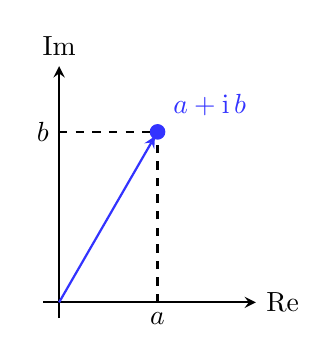
\begin{tikzpicture}[>=stealth,thick]
    \draw[->] (-0.2,0) -- (2.5,0) node[right]{Re};
    \draw[->] (0,-0.2) -- (0,3) node[above]{Im};
    \draw[->,blue!80,shorten >=-1pt]
    (60:2.5) node[fill,circle,inner sep=2pt,outer sep=0pt,label=above right:$a+\mathrm{i}\,b$]
    (z) {} (0,0) --(z);
    \draw[dashed] (0,0|-z) node[left]{$b$}-- (z)
  (0,0-|z) node[below]{$a$}-- (z);
  \end{tikzpicture}
  \end{center}
\end{frame}

\begin{frame}
  La norma d'un nombre complex es calcula fent $|(a+bi)|=\sqrt{a^2+b^2}$.

  Podem fer el següent producte:
  \[
    e^{i\theta}(x+iy)= (\cos{\theta}+i\sin{\theta})(x+iy)=(x\cos{\theta}-y\sin{\theta})+i(x\sin{\theta}+y\cos{\theta})
  \]
  Que es pot escriure com a la rotació en 2D del punt $(x,y)
  $:
  \[
    \begin{pmatrix}x'\\y'\end{pmatrix}=
    \begin{pmatrix}\cos{\theta}&-\sin{\theta}\\\sin{\theta}&\cos{\theta}\end{pmatrix}
    \begin{pmatrix}x\\y\end{pmatrix}
  \]
  El 1843, el matemàtic William R. Hamilton va descobrir que les rotacions tridimensionals es podien descriure amb una generalització dels nombres complexos anomenada {\bf quaternions}.
\end{frame}

\begin{frame}
  \frametitle{Àlgebra de quaternions}
  Un quaternió és una tupla de 4 valors que s'escriu formalment com $q_0+q_1i+q_2j+q_3k$, on $q_i \in \mathbb{R}$ i els símbols $i,j,k$ satisfan aquestes propietats:
  \begin{eqnarray*}
    i^2=j^2=k^2=-1\\
    \begin{matrix}ij=k&ji=-k\\
                  jk=i&kj=-i\\
                  ki=j&ik=-j
    \end{matrix}
  \end{eqnarray*}
  \begin{exercici}{}
    Troba les expressions de la suma i producte de dos quaternions.
  \end{exercici}
\end{frame}

\begin{frame}[allowframebreaks]
 \frametitle{Conjugat i norma}
 En {\bf nombres complexos}, el producte és commutatiu i cada nombre té un invers. Considerem el producte d'un nombre complex $z=a+bi$ pel seu conjugat $z^*=a-bi$:
 \begin{eqnarray*}
   (a+bi)(a-bi)&=&a^2 -b^2 i^2 = a^2+b^2\\
   \frac{(a+bi)(a-bi)}{a^2+b^2}=(a+bi)\frac{a-bi}{a^2+b^2}&=&1\\
   (a+bi)^{-1}&=&\frac{a-bi}{a^2+b^2}
 \end{eqnarray*}
 és a dir, que $z^{-1}=\frac{z^*}{\abs{z}^2}$ per a qualsevol nombre complex.
 En quaternions, el conjugat de $q=q_0+q_1i+q_2j+q_3k$ es defineix com
 \[
   q^*=q_0-q_1i-q_2j-q_3k
 \]
 i la seva norma és:
 \[
  \abs{q}=\sqrt{q_0^2+q_1^2+q_2^2+q_3^2}
 \]

  \begin{exercici}{}
    Mostra com, de manera anàloga als números complexes, cada quaternió no nul té un invers de la forma: $q^{-1}=\frac{q^*}{\abs{q}^2}$
  \end{exercici}

  \vspace{\baselineskip}
  El producte de quaternions {\bf no és commutatiu}.
\end{frame}

\begin{frame}
  \frametitle{Quaternions en rotacions}
  Un vector a $\mathbb{R}^3$ pot expressar-se com un quaternió pur, un quaternió que no té part real: $q=0+xi+yj+zk$. Podem definir un quaternió $q_R$ de norma 1 que representi la rotació del quaternió $q$ entre dues bases diferents $A$ i $B$ com:
 \small
  \begin{eqnarray}
    q_B&=& q_Rq_Aq_R^*\\\nonumber
                &=& (q_0+q_1i+q_2j+q_3k)(xi+yj+zk)(q_0-q_1i-q_2j-q_3k)\\\nonumber
                &=& (x(q_0^2+q_1^2-q_2^2-q_3^2)+2y(q_1q_2-q_0q_3)+2z(q_0q_2+q_1q_3))i+\\\nonumber
                &&  (2x(q_0q_3+q_1q_2)+y(q_0^2-q_1^2+q_2^2-q_3^2)+2z(q_2q_3-q_0q_1))j+\\\nonumber
                &&  (2x(q_1q_3-q_0q_2)+2y(q_0q_1+q_2q_3)+z(q_0^2-q_1^2-q_2^2+q_3^2))k
                \label{eq:quatrot}
  \end{eqnarray}
  \normalsize
  Tot i semblar enrevessat, és molt simple de programar i eficient (no inclou el càlcul de funcions trigonomètriques!).
\end{frame}

\begin{frame}
  \frametitle{Matriu de rotació a partir d'un quaternió}
  Podem expressar l'equació anterior en forma matricial i trobar la matriu de rotació entre la base $A$ i la $B$ fent:
  \[
    M=R_{A\rightarrow B}=2\cdot \begin{pmatrix}
    q_0^2+q_1^2-0.5 & q_1q_2-q_0q_3 & q_0q_2+q_1q_3 \\
    q_0q_3+q_1q_2 & q_0^2+q_2^2-0.5 & q_2q_3-q_0q_1 \\
    q_1q_3-q_0q_2 & q_0q_1+q_2q_3 & q_0^2+q_3^2-0.5
  \end{pmatrix}
  \]
  on hem usat que la norma del quaternió de rotació ha de ser 1: $\abs{q}=\sqrt{q_0^2+q_1^2+q_2^2+q_3^2}=1$.

  Notar que la rotació obtinguda a partir del quaternió $q$ és la mateixa que l'obtinguda a partir del quaternió $-q$.
\end{frame}

\begin{frame}
  \frametitle{Angle i eix de rotació a partir d'un quaternió i viceversa}
  Donat un quaternió unitari $\hat{q}=q_0+q_1i+q_2j+q_3k$, l'angle de rotació i l'eix associats són:
  \begin{eqnarray*}
    \theta &=& 2 \arccos{q_0}\\
    \hat{r}&=& \frac{(q_1,q_2,q_3)}{\sqrt{(1-q_0^2)}} = \left(
    \frac{q_1}{\sin{\frac{\theta}{2}}},
    \frac{q_2}{\sin{\frac{\theta}{2}}},
    \frac{q_3}{\sin{\frac{\theta}{2}}}
    \right)
  \end{eqnarray*}
  L'operació inversa seria:
  \[
    q=\cos{\frac{\theta}{2}}+i\sin{\frac{\theta}{2}}\hat{r}_x+j\sin{\frac{\theta}{2}}\hat{r}_y+k\sin{\frac{\theta}{2}}\hat{r}_z
  \]
  \begin{exercici}{}
    Quin és el quaternió de la rotació de 180 graus al voltant d'un eix qualsevol? i de rotar 0 graus? A partir d'aquests dos quaternions, fes l'operació inversa. Què passa si l'angle és 0 graus?
  \end{exercici}
  % q=0+ix+jy+kz q=1+0i+0j+0k
\end{frame}

\begin{frame}
  \frametitle{Quaternió a partir d'una matriu de rotació}
  \begin{enumerate}
    \item Primer, calculem la traça de la matriu $M$: $tr(M)=4q_0^2-1$ i obtenim $q_0=\sqrt{\frac{tr(M)+1}{4}}$.
    \item A partir de $M_{11}=2(q_0^2+q_1^2-0.5)$, obtenim $q_1=\sqrt{\frac{M_{11}}{2}+\frac{1-tr(M)}{4}}$
    \item A partir de $M_{22}=2(q_0^2+q_2^2-0.5)$, obtenim $q_2=\sqrt{\frac{M_{22}}{2}+\frac{1-tr(M)}{4}}$
    \item A partir de $M_{33}=2(q_0^2+q_3^2-0.5)$, obtenim $q_3=\sqrt{\frac{M_{33}}{2}+\frac{1-tr(M)}{4}}$
  \end{enumerate}
\end{frame}

\begin{frame}
  \frametitle{Quaternió a partir de tres angles d'Euler}
  Si considerem la rotació al voltant dels tres eixos:
  \scriptsize
  \[
   \begin{array}{ccc}
    M_{\psi}=\begin{pmatrix}
                            \cos{\psi}&-\sin{\psi}&0\\
                            \sin{\psi}&\cos{\psi}&0\\
                            0&0&1
             \end{pmatrix}
    &
    M_{\theta}=\begin{pmatrix}
                            \cos{\theta}&0&-\sin{\theta}\\
                            0&1&0\\
                            \sin{\theta}&0&\cos{\theta}
               \end{pmatrix}
    &
    M_{\phi}=\begin{pmatrix}
                            1&0&0\\
                            0&\cos{\phi}&-\sin{\phi}\\
                            0&\sin{\phi}&\cos{\phi}
               \end{pmatrix}
    \end{array}
  \]
  \normalsize
  i les fòrmules de la pàgina anterior obtenim:
  \[
    \begin{array}{ccc}
      q_{\psi}=\cos{\frac{\psi}{2}}+k\sin{\frac{\psi}{2}} &
      q_{\theta}=\cos{\frac{\theta}{2}}+j\sin{\frac{\theta}{2}} &
      q_{\phi}=\cos{\frac{\phi}{2}}+i\sin{\frac{\phi}{2}}
    \end{array}
  \]

  \begin{exercici}{}
    Rota amb quaternions el punt $(1,1,1)$ 60 graus al voltant de l'eix $Z$
  \end{exercici}
  \vspace{\baselineskip}
  Una web excepcional: \url{http://eater.net/quaternions}

\end{frame}

\begin{frame}
\frametitle{References}

\footnotesize{
\begin{thebibliography}{99} % Beamer does not support BibTeX so references must be inserted manually as below

\begin{columns}[t]
  \column{.45\textwidth}

\bibitem[VanVerth, 2015]{vanverth} James M. Van Verth, Lars M. Bishop (2015)
\newblock Essential Mathematics for Games and Interactive Applications
\newblock \emph{Elsevier}.

\bibitem[Lipschutz, 2001]{schaum} Seymour Lipschutz, Marc Lipson (2001)
\newblock Schaum's outlines: Linear Algebra (3rd Ed)
\newblock \emph{McGraw Hill}.

\column{.45\textwidth}

\bibitem[Riley, 2002]{riley} K.F. Riley, M.P. Hobson, S.J. Bence (2002)
\newblock Mathematical Methods for Physics and Engineering (2nd Ed)
\newblock \emph{McGraw Hill}.

\bibitem[García]{jlgarcia} Josep Lluís García
\newblock Presentacions Matemàtiques Grau en Multimèdia, Aplicacions i Videojocs
\newblock \emph{UVic-UCC}.

\bibitem[Corbera, 2015]{mcorbera} Montserrat Corbera, Vladimir Zaiats
\newblock Apunts d'Àlgebra Lineal (2015)
\newblock \emph{UVic-UCC}.

\bibitem[Calle, 2017]{mcalle} Malu Calle
\newblock Apunts d'Àlgebra Lineal (2017)
\newblock \emph{UVic-UCC}.

\end{columns}
\end{thebibliography}

}
\end{frame}
%----------------------------------------------------------------------------------------

\end{document}
